\documentclass[sn-mathphys-num]{sn-jnl}
\usepackage{graphicx}%
\usepackage{multirow}%
\usepackage{amsmath,amssymb,amsfonts}%
\usepackage{amsthm}%
\usepackage{mathrsfs}%
\usepackage[title]{appendix}%
\usepackage{xcolor}%
\usepackage{textcomp}%
\usepackage{manyfoot}%
\usepackage{longtable}%
\usepackage{booktabs}%
\usepackage{array}%
\usepackage{booktabs}%
\usepackage{algorithm}%
\usepackage{algorithmicx}%
\usepackage{algpseudocode}%
\usepackage{listings}%
\theoremstyle{thmstyleone}
\newtheorem{theorem}{Theorem}
\newtheorem{proposition}[theorem]{Proposition}
\theoremstyle{thmstyletwo}%
\newtheorem{example}{Example}%
\newtheorem{remark}{Remark}%
\usepackage{longtable}
\usepackage{booktabs}
\usepackage{array}
\usepackage{xcolor}
\usepackage{tcolorbox}
\theoremstyle{thmstylethree}%
\newtheorem{definition}{Definition}%

\raggedbottom

\bibliographystyle{elsarticle-num}

\usepackage{array}
\usepackage{tabularx}

\makeatletter
\renewcommand\subsubsection{%
  \@startsection{subsubsection}{3}{\z@}%
  {-3.25ex\@plus -1ex \@minus -.2ex}%
  {1.5ex \@plus .2ex}%
  {\normalfont\normalsize}}
\makeatother

\begin{document}

\title[Article Title]{SNR-Responsive Communication: Turbo Codes and BCH in a Dynamic HARQ Scheme for Enhanced Efficiency}

\author[1]{\fnm{C. } \sur{Gnana Jyothi}}\email{chinthagnanajyothi.221cs118@nitk.edu.in}
\author[2]{\fnm{P. } \sur{Chandana Sai Sri Hasitha}}\email{prathapachandanasaisrihasitha.221cs139@nitk.edu.in}
\author[3]{\fnm{N. } \sur{Yaswanth}}\email{namburiyaswanth.221cs232@nitk.edu.in}
\author*[4]{\fnm{B. R.} \sur{Chandavarkar}}\email{brc@nitk.edu.in}
	
\affil*[1]{\centering \orgdiv{Department of Computer Science and Engineering}, \\ \orgname{National Institute of Technology Karnataka, Surathkal}, \\ \orgaddress{\city{Mangaluru-575025}, \state{Karnataka}, \country{India}}}

\abstract{Wireless communication systems face many challenges due to fluctuating channel conditions, which lead to variable error rates and require robust error management tactics. Standard Automatic Repeat Request (ARQ) methods suffer from high communication overhead and latency and are inefficient in handling retransmissions. Although traditional HARQ is effective, its high implementation costs limit its widespread use. This underscores the need for adaptive systems that dynamically respond to changing channel conditions based on Signal-to-Noise ratio (SNR) values. This paper proposes the Dynamic  HARQ (D-HARQ) that switches between ARQ, HARQ with Bose-Chaudhuri-Hocquenghem (BCH) codes, and HARQ with turbo codes based on channel conditions during the transmission. Further, this paper incorporates a selective soft combining technique by estimating the receiver end's signal-to-noise ratio (SNR). The primary objective is to maximize throughput even at low SNR values while ensuring optimal complexity.}

\keywords{Adaptive HARQ, SNR estimation, Turbo codes, BCH codes, Selective soft combining, Error correction, Throughput optimization}

\maketitle

\section{Introduction}\label{s1}

Error control mechanisms are essential for ensuring reliable data transmission. They help detect errors and trigger retransmissions when packets are lost or corrupted. When data travel from one application to another, it goes through multiple steps and errors can occur at any stage, making error control a crucial part of maintaining communication quality\cite{r5}. Due to the necessity of numerous retransmissions, standard Automatic Repeat Request (ARQ) schemes fall short of adequately correcting all errors.  Thus, this paper leverages the technology of Hybrid ARQ (HARQ), which integrates ARQ with Forward Error Correction (FEC) \cite{r14, r13} for its enhanced efficiency in this context. However, this system may not be necessary under good channel conditions. This paper develops a novel approach to address this issue by adjusting to the varying needs of different channel conditions.

\subsection{Go-Back-N (GBN) Scheme } \label{s1.1}

GBN scheme \cite{r26} is one of the Pure ARQ methods. In this scheme, the sender transmits a sequence of frames without waiting for acknowledgment until it reaches a specified window size. If errors are detected or the packet is lost, a negative acknowledgment (NACK) \cite{r12}  is sent, and the sender resends all frames starting from the last acknowledged frame. Figure \ref{fig:1}  \cite{r12} illustrates the GBN scheme, where the sender (transmitter) transmits a sequence of frames (M1, M2, M3, ...) to the receiver. The receiver acknowledges the correctly received frames with ACK messages (ACK1, ACK2, ...). If a frame is lost or corrupted, the receiver sends a negative acknowledgment (NACK4 in the figure), prompting the sender to retransmit all frames starting from the lost frame (M4 in this case). This scheme does not require a storage buffer on the receiver side. GBN guarantees data integrity and reduces network congestion.

\begin{figure}[H]
    \centering
    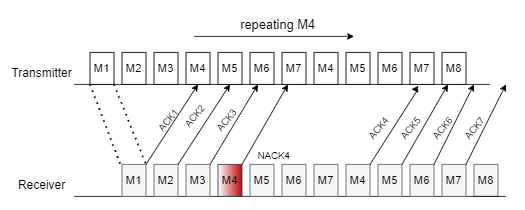
\includegraphics[width=0.8\textwidth]{gbn.png}
    \caption{Go Back-N (GBN) scheme}
    \label{fig:1}
\end{figure}

\subsection{Hybrid ARQ} \label{s1.2}

Hybrid ARQ \cite{r1, r50} combines ARQ with FEC, enabling error correction during transmission and reducing the likelihood of additional errors. If packet errors remain uncorrected, the system initiates retransmission. HARQ mainly has two basic schemes: firstly, Hybrid ARQ Type I, which has adaptive coding rates and additional error-correcting codes to minimize retransmissions while maintaining data integrity; Hybrid ARQ Type II uses redundancy to improve error correction capabilities later. These approaches guarantee robust data transmission, optimizing throughput, and reliable communication.
 
\subsection{Turbo Codes}  \label{s1.3}

Turbo codes \cite{r22} are a part of error-correcting codes that employ parallel concatenated convolutional codes to achieve remarkably efficient error correction. They are most commonly used in 3G/4G mobile communications (e.g., LTE) and in satellite communications, where there is a high demand for reliable information transfer. Turbo codes offer superior performance in noisy channels by iteratively decoding received signals. They take advantage of the redundancy provided by multiple convolutional codes in parallel. This iterative decoding process allows turbo codes to approach the Shannon limit. In Turbo codes, the code rate refers to the ratio of information bits to the total number of transmitted bits. The natural coding rate of a turbo code is R = 1/3 (three output bits for one input bit). 

\begin{figure}[H]
    \centering
    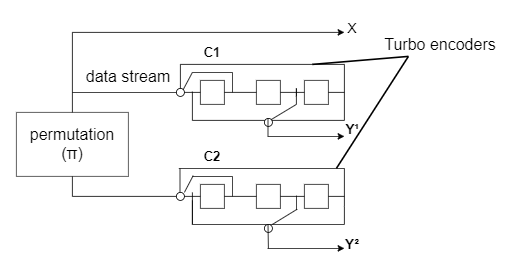
\includegraphics[width=0.8\textwidth]{Turbo_diagram.png}
    \caption{A classical Turbo code }
    \label{fig:12}
\end{figure}

Figure \ref{fig:12} \cite{r25} depicts a classical Turbo Code structure, which consists of the parallel concatenation of two binary  Convolutional encoders, C1 and C2, separated by a permutation block labeled $\pi$. The input data stream X is directly fed into the first encoder C1, producing the systematic output y1. The same input data X is also passed through the permutation block ($\pi$), which rearranges or interleaves the order of the data bits before feeding them into the second encoder C2, generating the parity output y2. Therefore, the Turbo Code encoder outputs are y1, which is an exact copy of the input data X (systematic output from C1), and y2, the parity output from C2, after interleaving the input data. The systematic and parity outputs (y1 and y2) are then transmitted. The key idea behind the Turbo Code structure is that the interleaved introduces redundancy and randomizes the input data, allowing the parallel encoders to provide robust error correction capabilities when decoding at the receiver end. Despite high error-correcting capability, they are quite complex to implement.

\subsection{Soft Combining \cite{r15}} \label{s1.4}

Soft combining stores a received erroneous packet in a buffer rather than discarding it. Two independently uncorrectable erroneous packets may be decoded correctly using the useful information obtained from their combination. This scheme has two main methods: chase combining and Incremental Redundancy (IR). In chase combining, all retransmissions are identical; using maximum-ratio combining the received bits with the error bits of previous transmissions adds extra energy for each retransmission by increasing the $Eb/N_0$ ratio. In incremental redundancy, the encoder generates distinct redundancy bits by puncturing its output, adding new information to each retransmission.

\begin{figure}[H]
    \centering
    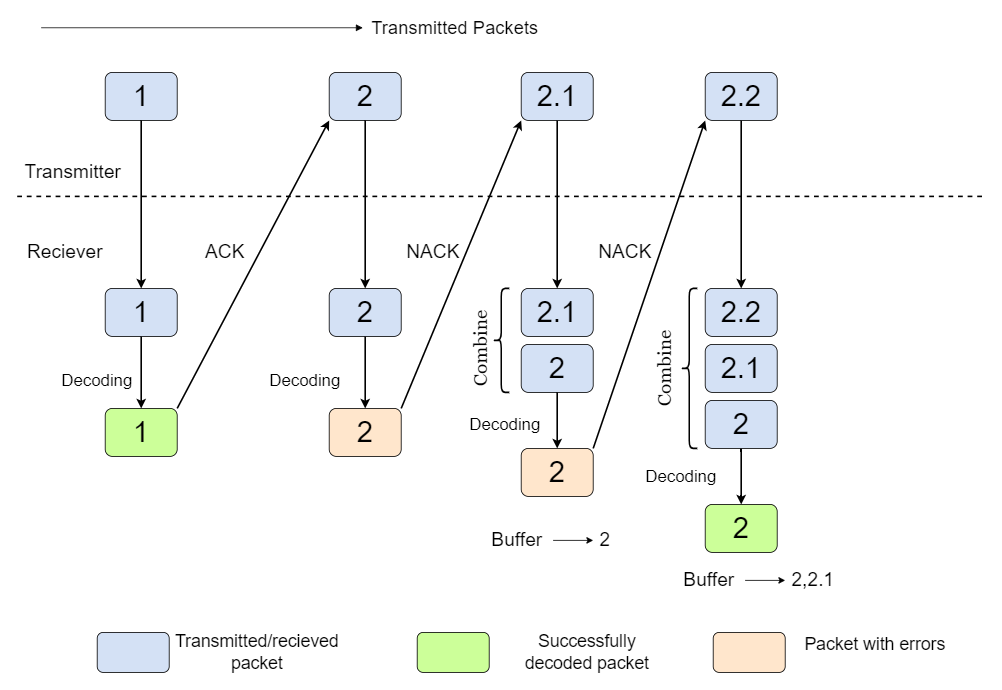
\includegraphics[width=0.8\textwidth]{Soft_Combining_3.png}
    \caption{Illustration of Soft combining with HARQ }
    \label{fig:10}
\end{figure}

Figure \ref{fig:10} \cite{r23} illustrates soft combining with HARQ in a communication system. The transmitter sends packets, and the receiver decodes them. If it correctly decodes a packet, it returns an ACK to the transmitter. If errors occur in the received packet, the receiver sends a NACK and stores it in a buffer. The transmitter then resends the new copy of the same packet, and the receiver combines (soft combining) the previously stored erroneous packet with the newly received packet to improve the decoding process. The receiver repeats the combining process for subsequent NACKs and retransmissions, storing the combined packets in the buffer (e.g., 2, 2.1, 2.2.1). The soft combining techniques enhance the reliability of data transmission by utilizing the information from previous erroneous transmissions, leading to improved error correction and overall system performance.

There are several existing error-correcting mechanisms available. Some are easy to implement but do not offer strong error correction capabilities, while others are complex but provide robust error correction. Therefore, FEC \cite{r14} should be chosen based on the channel conditions. Many existing approaches involve repeated retransmissions because they discard corrupted packets rather than utilizing them. These schemes are significant in DVB (Digital Video Broadcasting) and satellite communication systems \cite{r18}.

This paper enhances system efficiency by dynamically switching among ARQ, HARQ with Turbo Codes, and HARQ with BCH codes based on fluctuating SNR values. It introduces a novel mechanism for selective soft combining packets at the receiver end based on current channel conditions. This approach minimizes retransmissions by utilizing corrupted packets rather than discarding them. Selecting the appropriate schemes at every data transmission stage will result in significant throughput improvements across all scenarios. 

The paper is structured as follows: Section \ref{s2} covers the literature Survey, while Section \ref{s3} discusses the design and implementation of the proposed approach. Section \ref{s4} presents simulation results, analysis, and comparisons with existing methods. Finally, Section \ref{s5} concludes with future directions and references.

\section{Literature survey} \label{s2}

Subsections 2.1 to 2.7 outline various techniques, along with their strengths and limitations, from different papers focused on enhancing data transmission efficiency and reliability using HARQ methods. Subsection \ref{s2.1} discusses Adaptive HARQ with Reed-Solomon (RS) Codes. Subsection \ref{s2.2} covers Adaptive HARQ with Two RS Codes. Subsection \ref{s2.3} focuses on Adaptive HARQ with BCH Codes. Subsection \ref{s2.4} highlights Non-orthogonal HARQ for URLLC. Subsection \ref{s2.5} is about Energy-efficient optimization over fading channels. Subsection \ref{s2.6} covers Adaptive HARQ with reinforcement learning technique. Finally, Subsection \ref{s2.7} discusses data recovery loops in 6G networks.

\subsection{Adaptive HARQ with Reed-Solomon codes} \label{s2.1}

J. P. Peter Fidler et al. \cite{r6} introduced the adaptation rule that employs a straightforward approach based on counting consecutive acknowledgments (ACKs) and negative acknowledgments (NACKs) to dynamically switch between HARQ and ARQ modes, depending on the predicted channel state. As depicted in  Figure \ref{fig:2} \cite{r6}, the key component of this model is the threshold parameter (T), which sets a limit on consecutive ACKs required to transition from HARQ to ARQ mode. Once the number of consecutive ACKs exceeds this threshold, the system shifts to the less complex ARQ mode, signifying a stable channel condition. If a NACK is detected, the system immediately switches back to HARQ mode to improve error correction as the channel degrades.

\begin{figure}[H]
    \centering
    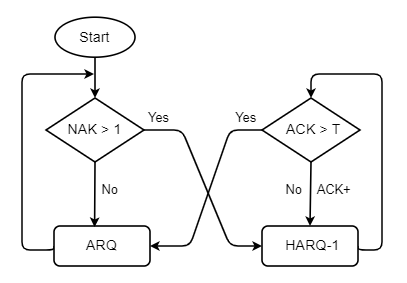
\includegraphics[width=0.6\textwidth]{rs.png}
    \caption{Adaptive HARQ using RS codes}
    \label{fig:2}
\end{figure}

This approach has several benefits. First, its adaptive nature allows a quick switch to HARQ mode when a noisy channel is detected. This dynamic approach requires a threshold of positive acknowledgments to switch back to ARQ mode, ensuring that the system remains robust and responsive to real-time channel conditions. On the other hand, this schema has a few limitations, such as limited adaptability with only two states, which restricts the system adjustment to high fluctuations in channel quality and limited scalability for complex network environments.

\subsection{Adaptive HARQ with two RS codes} \label{s2.2}

Michal M. et al. \cite{r8} proposed a three-stage adaptive ARQ/HARQ1/HARQ2 scheme. Increasing the number of states compared to the adaptive HARQ scheme discussed in \ref{s2.1} allows for higher throughput for various channel bit error rates. There are three operating modes: pure ARQ -Go Back -N \cite{r18}, HARQ1 with RS code (511, 383, 64), and HARQ2 with RS code (511, 255, 128).  The transmitter follows the pure ARQ method for state L with a low channel error rate. The high channel error rate is further divided into HARQ1 and HARQ2. Both states use RS codes with different code rates.

Figure \ref{fig:3} \cite{r8} illustrates the switching logic, where the transmitter controls the transition from ARQ to HARQ modes or between HARQ1 and HARQ2. Meanwhile, the receiver manages the switch from HARQ modes back to ARQ. In the proposed approach \cite{r8}, these three confirmations are utilized as follows:

   \begin{itemize}
       \item The receiver sends an ACK when the packet contains no errors (pure ARQ) or when the RS code can correct the packet (HARQ1, HARQ2).
       \item NAK when the RS code cannot rectify the packet (HARQ1, HARQ2).
       \item  ACK+   When there is no error in the previous W packets.
   \end{itemize}

   
\begin{figure}[H]
    \centering
    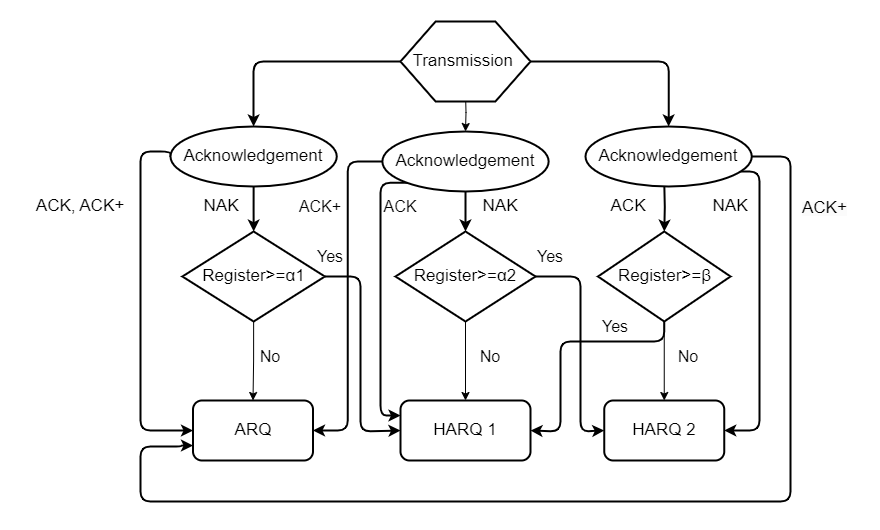
\includegraphics[width=0.9\textwidth]{two_rs.png}
    \caption{Dynamic Adaption of different HARQ schemes using two RS codes}
    \label{fig:3}
\end{figure}

This approach brings several advantages; firstly, it introduces a pioneering approach through a 3-stage proposal with a sliding window mechanism. Unlike conventional ARQ-HARQ methods with fewer stages, this multi-stage scheme offers flexibility and adaptability to diverse channel conditions. However, this approach fails to optimize throughput for a broader range of SNR values -also, limited capability in correcting random errors due to its RS error-correcting code.

\subsection{Adaptive HARQ with BCH codes } \label{s2.3}

F. C. Kvetoslava Kotuliakova et al. \cite{r5} presented an enhanced adaptive ARQ-HARQ method that uses BCH codes to improve the effectiveness of data transmission over varying channel conditions. This scheme dynamically modifies transmission schemes in response to the channel's measured bit error rate. This paper proposes an adaptive HARQ model that dynamically switches between HARQ1 and HARQ2 schemes, which have different code rates based on the estimated channel state. If the error rate is low, the GBN scheme is used, which is more efficient for good channel conditions. Otherwise, it evaluates the channel condition based on the number of NACKs and a predefined threshold. If the condition indicates significant transmission errors, the system follows the HARQ2 scheme with a higher code rate, enhancing reliability in challenging environments. The HARQ1 scheme with a medium code rate is used if the error level remains within an acceptable range.

% \begin{figure}[H]
%     \centering
%     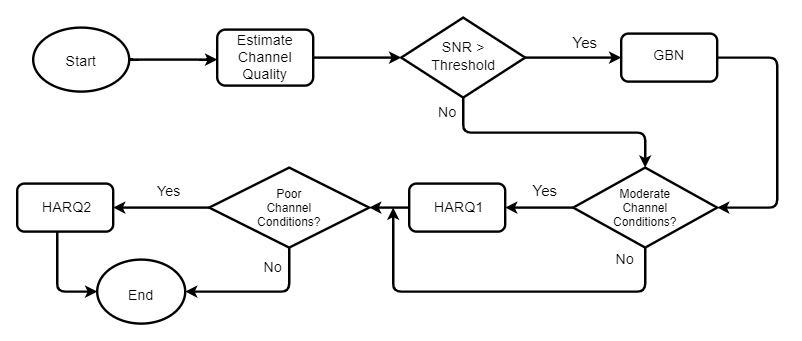
\includegraphics[width=0.9\textwidth]{bch_t.png}
%     \caption{Adaptive HARQ using BCH codes}
%     \label{fig:4}
% \end{figure}

These hybrid schemes combine two BCH codes selected to improve error correction performance in various channel conditions. The GBN \cite{r18} protocol is used for retransmissions, ensuring better performance, as discussed in Subsection \ref{s1.1}. This scheme has various advantages, including dynamically altering parameters to adapt to changing network conditions and effectively controlling retransmissions, significantly lowering latency and improving responsiveness. The disadvantage of this schema is the difficulty of maintaining effective data transmission under low SNR conditions. In such conditions, there is almost zero throughput.

\subsection{Non-orthogonal HARQ for URLLC} \label{s2.4}

Faisal Nadeem et al. \cite{r28} proposed the non-orthogonal HARQ for URLLC, a scheme tailored for ultra-reliable and low-latency communication systems. It introduces non-orthogonal retransmissions, allowing multiple packets to share time slots during retransmission, significantly reducing latency. This scheme is particularly successful in high-speed applications, such as industrial automation or driverless cars. While it achieves impressive reliability and delay reductions, its reliance on non-orthogonal resource sharing can lead to resource allocation complexities in highly dynamic network environments. Additionally, its application is primarily limited to latency-critical scenarios.

\subsection{Energy-efficient optimization for HARQ schemes over time-correlated fading channels} \label{s2.5}

Zheng Shi et al. \cite{r29} proposed an energy-efficient optimization for HARQ schemes in the context of time-correlated fading channels, addressing the critical trade-off between energy consumption and communication reliability. The study improves energy efficiency by optimizing transmission powers and rates while maintaining acceptable performance in terms of error rates. The closed-form solutions derived for HARQ schemes, such as Type I, Chase Combining (CC), and Incremental Redundancy (IR), demonstrate a practical approach to reducing energy usage. However, the model assumes relatively stable time-correlated fading channels, which might not generalize well to rapidly changing SNR conditions. Moreover, the focus on energy efficiency sometimes comes at the cost of reduced throughput in highly challenging channel conditions.

\subsection{Adaptive HARQ with reinforcement learning} \label{s2.6}

Chia-Hung Yeh et al. \cite{r30} proposed the adaptive HARQ with reinforcement learning that employs machine learning to dynamically select optimal transmission strategies based on channel quality indicators (CQI). The approach uses reinforcement learning algorithms, to adapt to real-time changes in channel conditions by exploring an extensive action space, including varying retransmission schemes. This adaptability reduces block error rates and lower transmission delays compared to static HARQ mechanisms. Despite its strengths, this scheme introduces significant computational overhead, making it less feasible for real-time applications with resource-constrained devices. Additionally, the training phase for reinforcement learning models requires extensive data and computational resources, which might not always be practical.

\subsection{Data recovery loops in 6G networks} \label{s2.7}

Uyoata E. Uyoata et al. \cite{r31} presented the data recovery loops in a 6G networks paper that focuses on the interplay between HARQ schemes in the physical and medium access control layers and higher-layer ARQ mechanisms. This study emphasizes the need for enhanced coordination between layers to achieve efficient data recovery in 6G networks. The proposed enhancements, such as fast HARQ schemes for challenging radio conditions, show substantial throughput gains, especially for users at cell edges or with poor signal quality. However, the study narrows its scope to 6G scenarios, offering limited insights into how these mechanisms perform in legacy or non-6G network environments. The high complexity of integrating these multi-layer recovery loops also raises concerns about scalability and implementation in real-world systems.


\setlength{\tabcolsep}{4pt}
\setlength{\extrarowheight}{-2pt} % Adjust value as needed
\renewcommand{\arraystretch}{0.5}

\begin{longtable}{|>{\centering\arraybackslash}m{3.2cm}|>{\centering\arraybackslash}m{4.3cm}|>{\centering\arraybackslash}m{3.75cm}|>{\centering\arraybackslash}m{3.75cm}|}
\caption{Comparision of different HARQ techniques} \label{tab:3} \\ \hline
\textbf{Technique} & \textbf{Description} & \textbf{Advantages} & \textbf{Drawbacks} \\ 
\hline
\endfirsthead
\hline
\textbf{Technique} & \textbf{Description} & \textbf{Advantages} & \textbf{Drawbacks} \\ 
\hline
\endhead
\hline
\endfoot

Adaptive HARQ with Reed-Solomon (RS) Codes \cite{r6} & Dynamically switches between HARQ and ARQ modes based on ACKs and NACKs. & 
\begin{itemize}
    \item Robust and straightforward to channel fluctuations.
    \item Adapts quickly to noisy channels.
\end{itemize} & 
\begin{itemize}
    \item Limited adaptability with only two states.
    \item Poor scalability for complex networks.
\end{itemize} \\ 
\hline

Adaptive HARQ with Two RS Codes \cite{r8}& Employs a three-stage ARQ/HARQ1/HARQ2 scheme with different RS code rates. & 
\begin{itemize}
    \item Flexible and adaptable to diverse channel conditions.
    \item Higher throughput for various error rates.
\end{itemize} & 
\begin{itemize}
    \item Increased latency for real-time traffic.
    \item Limited error correction for random errors due to RS code design.
\end{itemize} \\ 
\hline

Adaptive HARQ with BCH Codes \cite{r5} & Dynamically switches between HARQ1 and HARQ2 schemes with varying code rates. & 
\begin{itemize}
    \item Adapts to moderate to high error rates effectively.
    \item Reduces latency by dynamically altering retransmission parameters.
\end{itemize} & 
\begin{itemize}
    \item Ineffective under low SNR conditions.
    \item Throughput approaches zero in poor signal environments.
\end{itemize} \\ 
\hline

Non-orthogonal HARQ for URLLC \cite{r28}& Introduces non-orthogonal retransmissions to reduce latency, enabling multiple packets to share time slots during retransmission. & 
\begin{itemize}
    \item Reduces latency.
    \item Effective in high-speed applications (e.g., autonomous vehicles, industrial automation).
\end{itemize} & 
\begin{itemize}
    \item Resource allocation complexities in dynamic networks.
    \item Limited versatility for throughput optimization.
\end{itemize} \\ 
\hline

Energy-efficient optimization over fading channels \cite{r29} & Optimizes transmission powers and rates for energy efficiency while maintaining reliability in time-correlated fading channels. & 
\begin{itemize}
    \item Enhances energy efficiency.
    \item Provides practical closed-form solutions for various HARQ schemes (e.g., Type I, CC, IR).
\end{itemize} & 
\begin{itemize}
    \item Assumes stable fading conditions.
    \item May reduce throughput in challenging channel environments.
\end{itemize} \\ 
\hline

Adaptive HARQ with reinforcement learning \cite{r30} & It uses machine learning to select optimal retransmission strategies based on channel quality indicators dynamically. & 
\begin{itemize}
    \item Adapts to real-time channel changes.
    \item Reduces block error rates and delays compared to static HARQ mechanisms.
\end{itemize} & 
\begin{itemize}
    \item High computational overhead.
    \item Requires extensive data and resources for model training.
\end{itemize} \\ 
\hline

Data recovery loops in 6G networks \cite{r31}& Enhances coordination between physical, MAC, and higher-layer ARQ mechanisms to improve data recovery in 6G networks. & 
\begin{itemize}
    \item Substantial throughput gains for edge users or poor signal quality.
    \item Effective in challenging radio conditions.
\end{itemize} & 
\begin{itemize}
    \item Limited applicability to non-6G systems.
    \item High complexity and scalability challenges in real-world implementations.
\end{itemize} \\ 
\hline

\end{longtable}

However, most solutions involve trade-offs between complexity, generalizability, and resource constraints, as mentioned in Table \ref{tab:3}, which should be carefully considered based on the intended application. The proposed D-HARQ perfectly balances complexity and throughput as it adaptively switches between schemes according to channel conditions, requiring no heavy computations.

\section{Design and Implementation of Dynamic HARQ (D-HARQ)} \label{s3}

This section of the paper discusses the design and implementation of the D-HARQ scheme to improve communication efficiency. Firstly, Subsection \ref{s3.1} provides insights into throughput analysis for schemes, including pure ARQ, HARQ with BCH, and turbo codes, explaining their performance under varying channel conditions. Secondly, Subsection \ref{s3.2} outlines a dynamic switching scheme between HARQ modes and pure ARQ based on NACK/ACK counts and SNR thresholds. Thirdly, Subsection \ref{s3.3} delves into the mechanism of HARQ with Turbo Codes, emphasizing error correction and throughput improvement in low SNR scenarios. Fourthly, in Subsection \ref{s3.4}, the SNR estimation algorithm based on Error Vector Magnitude (EVM) analysis is discussed, which is crucial for a selective soft combining scheme. Lastly, Subsection \ref{s3.5} discusses decision-making for soft combining at the receiver end.

D-HARQ dynamically adapts to different schemes based on real-time fluctuations in SNR values. When SNR is very low, it switches to robust turbo codes with HARQ for error correction. Conversely, when SNR is moderate to high, it employs  HARQ with BCH codes of different code rates. Notably, when the SNR reaches an extremely high value, the scheme strategically switches back to pure ARQ to reduce unnecessary complexity. The scheme operates in four states:  Pure ARQ with Go-back-N, two enhanced BCH codes HARQ1(4599, 3447) and HARQ2(4599, 2295), and an optimal state using HARQ with Turbo codes.

\subsection{Throughput of different schemes} \label{s3.2}

The first stage of implementation is a calculation of the throughput of different schemes like Pure ARQ, HARQ with BCH code, and HARQ with turbo codes. If the transmitter follows pure ARQ with the GBN scheme, then the throughput is given by Eq. \ref{6} \cite{r8}. Error detection bits multiply this throughput by the weight, i.e., the ratio of message symbols to the total number of symbols.

\begin{equation}\label{6} 
    \eta_{\text{L}} = \frac{1 - P_e}{1 + S \cdot P_e} \cdot \frac{N - CRC}{N} 
\end{equation} 

Here, $N$ is the length of the block, CRC represents the number of redundancy symbols added for error detection, ${P}_e$ is the probability of occurrence of an error in the packet in the pure ARQ method. ${P}_e$ depends on the channel bit error rate, burst errors, and block length, as expressed in Eq. \ref{7} \cite{r5}.
 
\begin{equation}\label{7} 
    P_e = 1 - (1 - P_b)^K
\end{equation}

Here, ${P}_b$ is the bit error rate, $K$ represents the number of information symbols in the packet, and S is defined as the ratio of the acknowledgment time delay to the block transmission time.

\begin{equation}\label{8}
     S = T_a / T_b
\end{equation}

${T}_a$ is the time delay of acknowledgment, defined as the delay from terminating block transmission to receiving and processing block acknowledgment. ${T}_b$ is the time of block transmission \cite{r21}.

If the transmission is in the HARQ scheme, the throughput \cite{r21} will be as follows :

\begin{equation}\label{10}
    \eta_H = \frac{K}{N} \times \frac{1 - \sum_{i=t+1}^{N} \binom{N}{i} P_s^i (1-P_s)^{N-i}}{1 + S \cdot \sum_{i=t+1}^{N} \binom{N}{i} P_s^i (1-P_s)^{N-i}}
\end{equation}

Here, t represents the count of repairable symbols (2t = redundancy bits), and ${P}_s$ is the probability that the symbol has an error, calculated as follows.
 
\begin{equation}\label{11}
    P_s = 1 - (1 - P_b)^b
\end{equation}

Here, b is no.of bits per symbol given by
\begin{equation}\label{9}
    b = \log_2(N+1)
\end{equation}

If the scheme uses turbo codes with a code rate of 1/3 for error correction, then the throughput is calculated as follows:

\begin{equation}
    T_{\text{hr}} = \left(\frac{R_{c}}{T_{r}}\right) \cdot \left(\frac{k}{k + n_{p}}\right)
\end{equation}

Where k/(k + ${n}_p$) is the fractional throughput loss because of additional parity bits added for detecting errors, where k represents the number of information bits, while  ${n}_p$ denotes the number of parity bits, ${R}_c$ denotes the code rate (here, ${R}_c$ =  1/3). ${T}_r$ represents the average number of transmissions in the HARQ scheme and is expressed in \cite{r19}.

\begin{equation}
    T_{r} = \sum_{i=0}^{\infty} P(D_{d})^{i} = \frac{1}{1 - P(D_{d})}
\end{equation} 

Where P(${D}_d$) is the probability that errors are present in the decoded packet.

\subsection{Switching Scheme} \label{s3.3}

This subsection explains the dynamic switching mechanism of the D-HARQ model between different modes and the calculation of thresholds for switching. Initially, the pure ARQ with GBN technique serves as the starting point. Once the number of transmitted packets reaches the size of the sliding window, decisions are made based on the counts of NACKs (Negative Acknowledgments) and ACKs (Acknowledgments) to determine whether a state transition is necessary.

The switching points are determined by identifying the SNR (signal-to-noise ratio) values at which both schemes yield identical throughput. The system transitions to the scheme with the higher throughput for subsequent SNR values until it reaches another switching point. However, under very low SNR conditions (0-3.47 dB), these schemes produce negligible throughput (nearly zero), as demonstrated in Section \ref{s4}. This paper addresses this limitation by introducing a key enhancement that involves the use of turbo codes.

\subsubsection{Turbo Codes for Low SNR Conditions}

When neither a positive acknowledgment (ACK) nor a NACK is received, it indicates a scenario of extremely low SNR, resulting in negligible throughput. This behavior is supported by the throughput formula, which is inversely proportional to parameter $S$, defined as the ratio of acknowledgment delay to block transmission time. Without acknowledgments, acknowledgment latency increases dramatically, pushing $S$ closer to infinity. As a result, throughput approaches zero, emphasizing the need for turbo codes in such situations. Using turbo codes in these circumstances significantly increases throughput.

\begin{figure}[H]
    \centering
    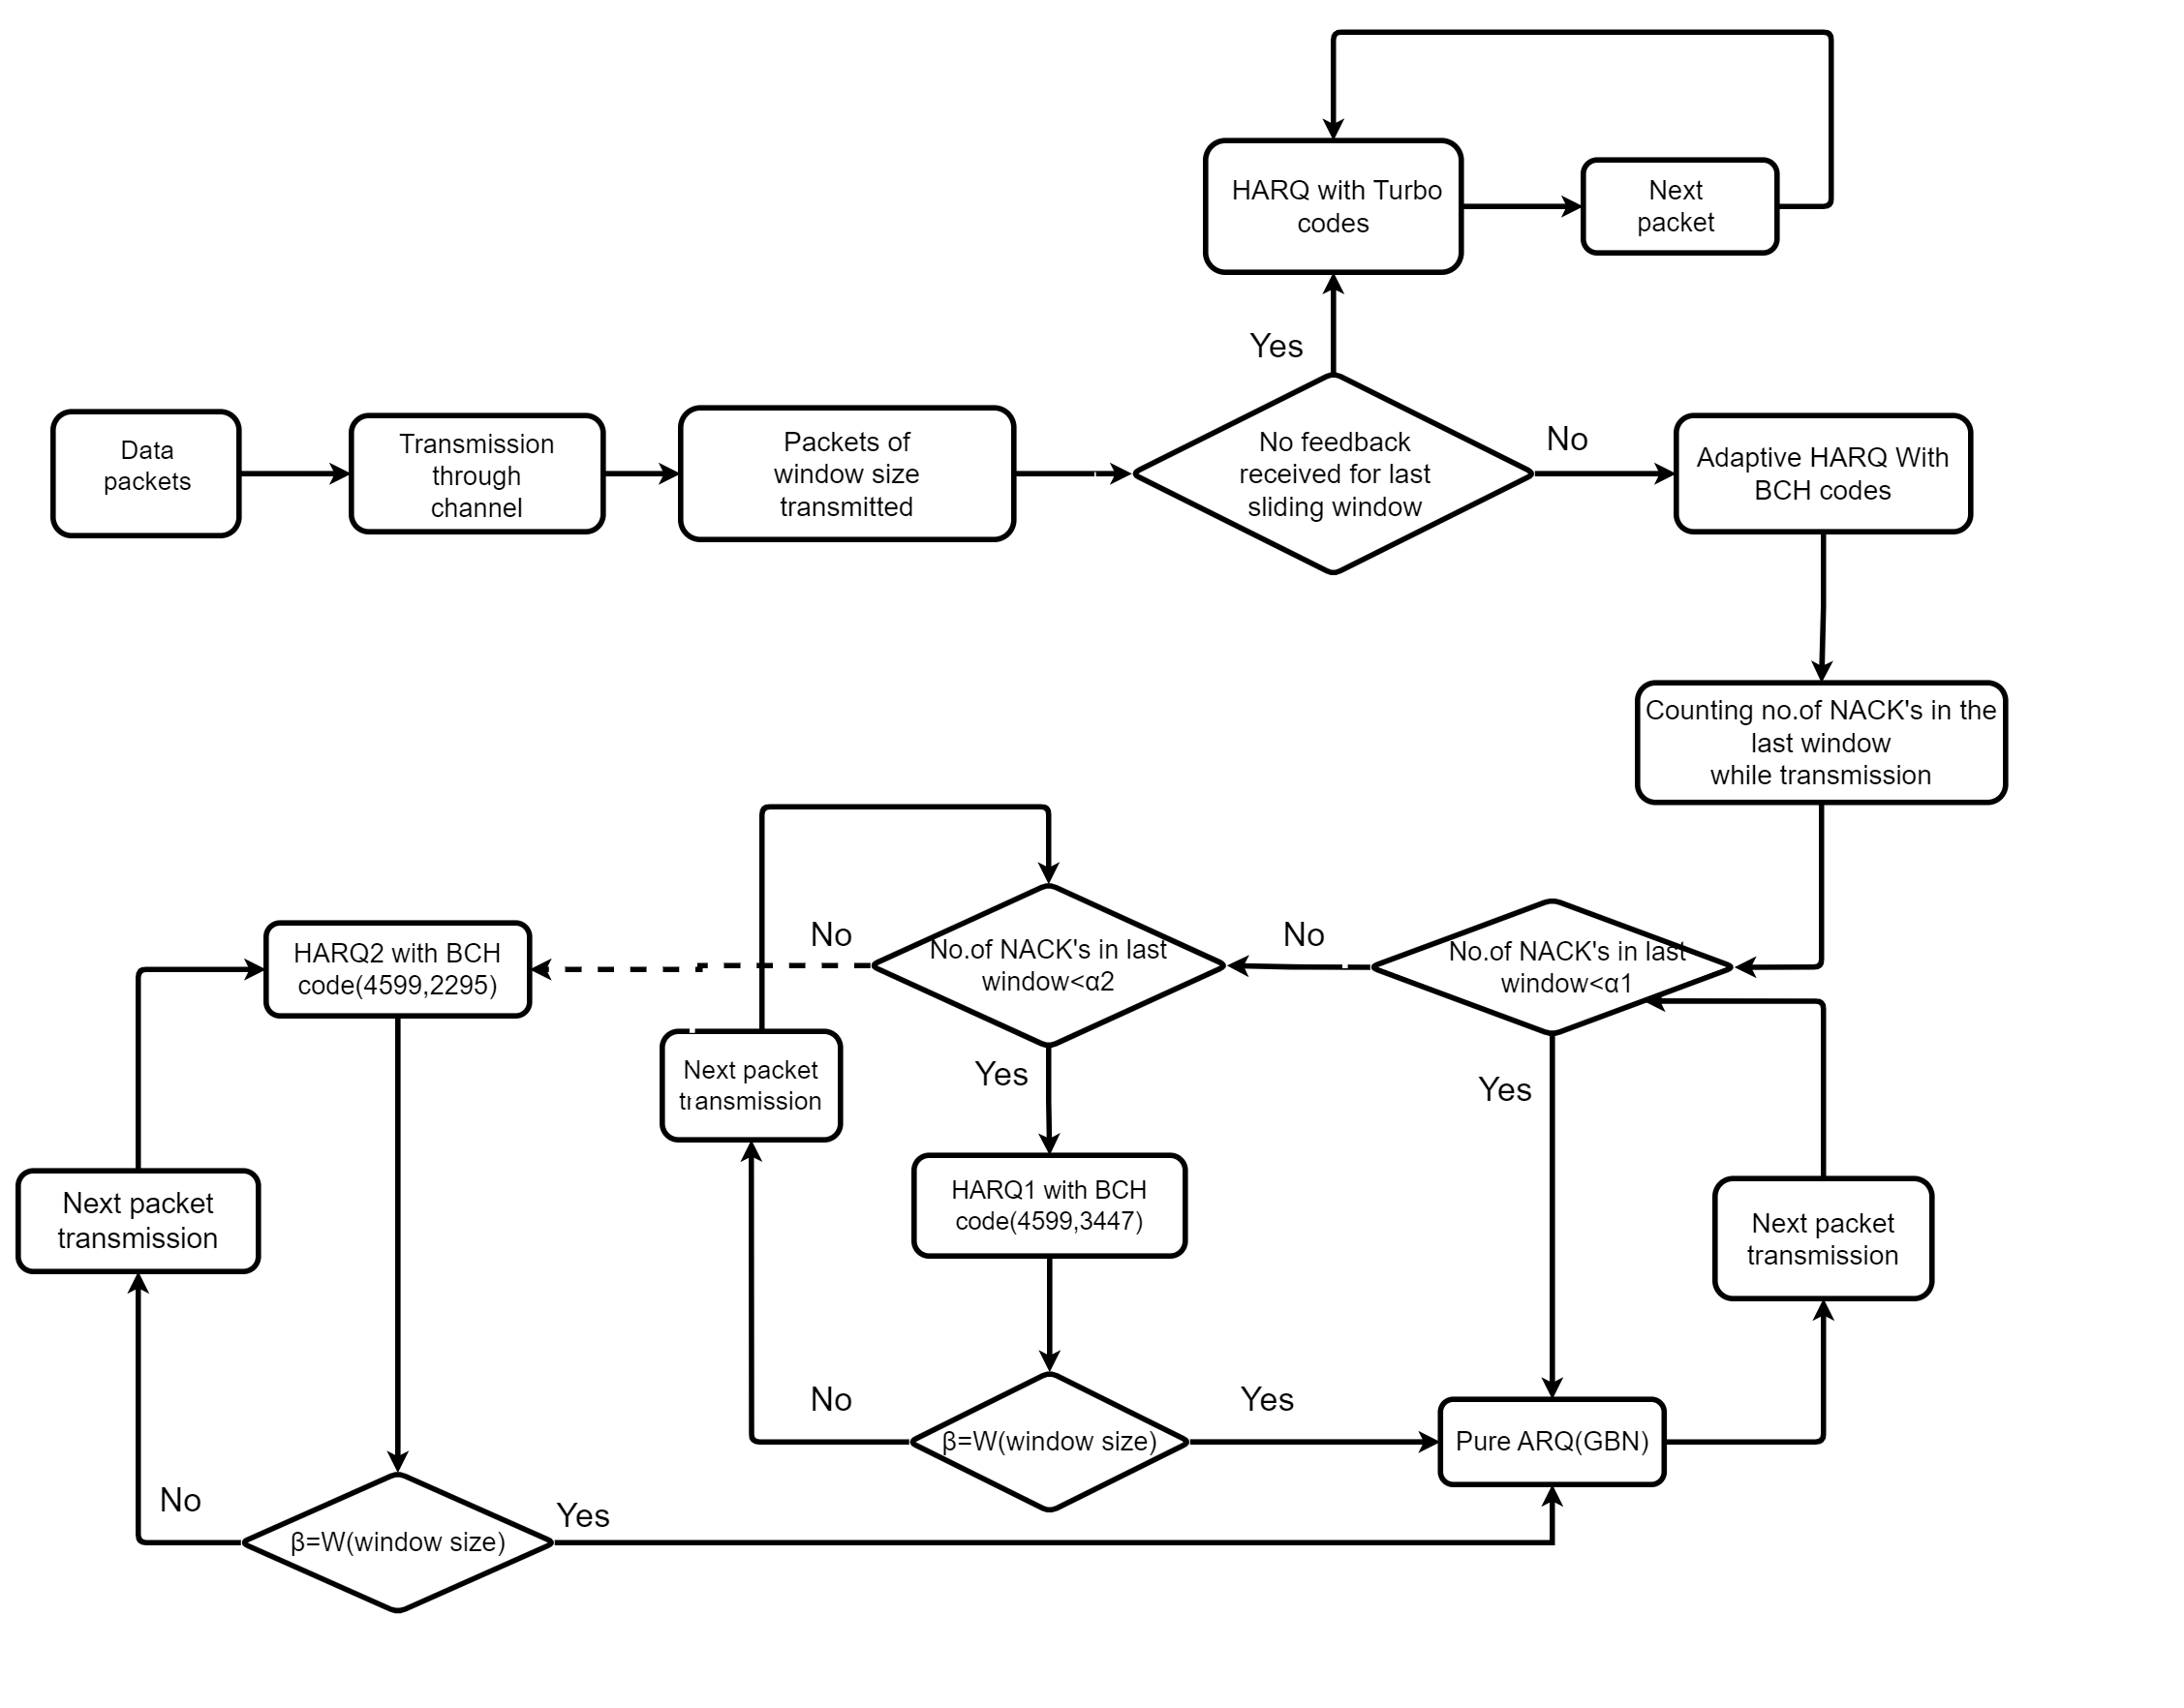
\includegraphics[width=\textwidth]{SWITCH.png}
    \caption{Illustration of the dynamic switching between different HARQ schemes}
    \label{fig:5}
\end{figure}

\subsubsection{Switching Criteria}

The number of NACKs governs the switching mechanism received within a sliding window. If the count of NACKs exceeds a threshold, $\alpha_1$, the scheme transitions from ARQ to HARQ1, as illustrated in Figure \ref{fig:5}. To compute $\alpha_1$, the throughput of ARQ is equated to that of HARQ1:

\begin{equation}
\frac{1 - P_e}{1 + S \cdot P_e} \cdot \frac{N \cdot b - CRC}{N \cdot b} = \frac{K}{N} \times \frac{1 - \sum_{i=t+1}^{N} \binom{N}{i} P_s^i (1-P_s)^{N-i}}{1 + S \cdot \sum_{i=t+1}^{N} \binom{N}{i} P_s^i (1-P_s)^{N-i}} \label{14}
\end{equation}

The parameters used in this Eq. \ref{14} are defined as follows. $P_e$ represents the probability of error in the packet in the pure ARQ, while ${P}_s$ is the probability that the symbol has an error. $N$ is the block length, representing the number of symbols in each packet, and $b$ is the number of bits per symbol in each block. $CRC$ represents the number of redundancy bits added for error detection. $S$ is the ratio of acknowledgment delay to block transmission time, defined as $S = \frac{T_a}{T_b}$, where $T_a$ is the acknowledgment delay, and $T_b$ is the time required to transmit a block. Moreover, $K$ represents the number of information symbols in the packet.

The unknown variable \(P_b \) (bit error probability) is determined by substituting the relevant formulas with \(P_e \) and \(P_s \). After determining \(P_b \), we derive \(P_e \) and determine the threshold \(\alpha_1 \) \cite{r8}.

\begin{equation}
    \alpha_1 = P_e \cdot W
\end{equation}

Where $W$ represents the sliding window size.

To compute the threshold $\alpha_2$ for switching from HARQ1 to HARQ2, we equate the throughput expressions of both schemes.

\begin{equation}
\frac{K_1}{N} \times \frac{1 - \sum_{i=t+1}^{N} \binom{N}{i} P_s^i (1-P_s)^{N-i}}{1 + S \cdot \sum_{i=t+1}^{N} \binom{N}{i} P_s^i (1-P_s)^{N-i}} = \frac{K_2}{N} \times \frac{1 - \sum_{i=t+1}^{N} \binom{N}{i} P_s^i (1-P_s)^{N-i}}{1 + S \cdot \sum_{i=t+1}^{N} \binom{N}{i} P_s^i (1-P_s)^{N-i}} \label{eq:combined2}
\end{equation}

Additional parameters introduced here include $K_1$, representing the number of information symbols in HARQ1, and $K_2$, denoting the number of information symbols in HARQ2.

This equation determines $P_s$, and the threshold $\alpha_2$ \cite{r8} is given by:

\begin{equation}
\alpha_2 = P_s \cdot W
\end{equation}

\subsubsection{Transition Back to ARQ}

When the last sliding window detects no errors, the receiver sends a new acknowledgment type, ACK+, to the transmitter. This triggers a transition from HARQ1 or HARQ2 to ARQ, as shown in Figure \ref{fig:5}. The transition depends on the number of consecutive ACKs received. The threshold for this scenario, $\beta$ \cite{r8}, is defined as:

\begin{equation}
\beta = W
\end{equation}

Where $\beta$ denotes the successful and error-free acknowledgment of every packet in the sliding window, this change improves system efficiency by reducing unnecessary computing overhead when channel conditions are favorable.

\subsubsection*{Summary of Switching Scheme}

The adaptive switching process ensures optimal throughput across varying SNR conditions. Turbo codes significantly improve performance under extremely low SNR (0-3.47 dB), as shown in Figure \ref{fig:6}. The proposed model balances complexity and efficiency by dynamically selecting the appropriate HARQ scheme based on channel conditions.

\subsection{Detailed mechanism of HARQ with Turbo Codes} \label{s3.4}

This subsection explains the mechanism of HARQ with turbo codes in the D-HARQ model. Initially, the packet goes through a series of encoding phases to improve error correction capabilities. As shown in Figure \ref{fig:15}, the first phase, known as Bit Splitting, prepares the input bitstream for parallel processing. Constituent follows this Encoding 1, where the first half of the bitstream is convolutionally encoded, introducing redundancy that serves as the foundation for error correction. To further improve the ability to correct errors, the bitstream undergoes interleaving, ensuring a more uniform distribution of potential errors. The process continues with Constituent Encoding 2, adding a layer of redundancy through a second convolutional encoder. Finally, Rate Matching is applied to adjust the encoded bitstream according to the transmission channel's bandwidth and error characteristics. Upon completing the encoding stages, the data is ready for modulation onto a carrier signal and transmitted across the communication channel, which is prone to noise and interference. At the receiving end, the Reception and Signal Demodulation stage takes over, where the transmitted signal is captured and demodulated to retrieve the encoded data bitstream.

\begin{figure}[H]
    \centering
    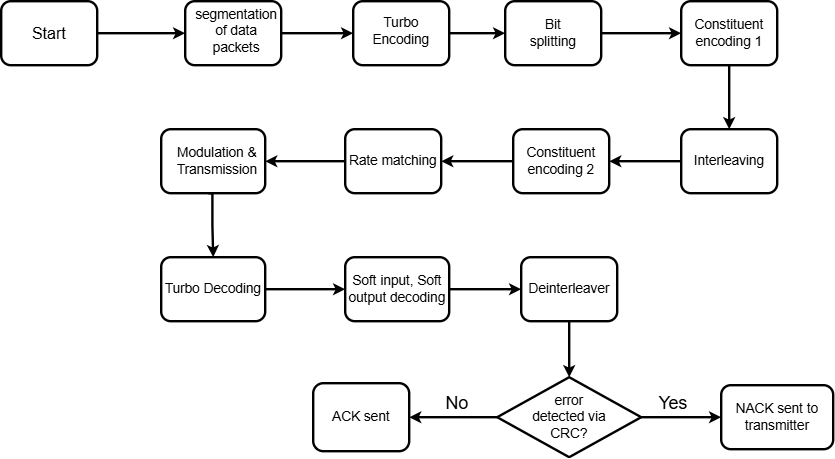
\includegraphics[width=\textwidth]{HARQ with Turbo codes.drawio.png}
    \caption{HARQ with Turbo codes}
    \label{fig:15}
\end{figure}

Soft-input Soft-output Decoding Iteration 1 is the first step in the turbo decoding process, as shown in Figure \ref{fig:15}. This phase represents the first attempt to decode the received signal by using soft decision inputs to generate soft decision outputs. These outputs, which contain probability metrics indicating the precision of each bit, significantly increase the effectiveness of the decoding process. The De-interleaver reorders bits between decoding iterations. Subsequent iterations of decoding are required to refine the accuracy of the data. After decoding, the Cyclic Redundancy Check (CRC) finds problems. If errors are discovered, it sends a NACK requesting retransmission; otherwise, it sends an Acknowledgement (ACK) indicating successful reception.

\subsection{SNR estimation algorithm} \label{s3.1}

This subsection presents a detailed explanation of the SNR estimation algorithm, a key part of the selective soft combining process. The Error Vector Magnitude (EVM) SNR estimation algorithm \ref{alg:snr_estimation} enhances the accuracy and scope of SNR estimation. This advancement comes in response to the limitations of current methodologies, which struggle with accurately estimating low SNRs. Eq. \ref{1} and Eq. \ref{2} initially calculate the mean and variance of the received signal samples $|y_n|$ at time instants n = 1, 2, ..., L after downsampling.

\begin{equation}\label{1} 
\text{mean} = \frac{1}{L} \sum_{n=1}^{L} |y_n|
\end{equation}

\begin{equation}\label{2} 
\text{var} = \frac{1}{L} \sum_{n=1}^{L}( |y_n| -\text{mean})^2
\end{equation}

SNR is calculated from Eq. \ref{3} \cite{r20} using these results.

\begin{equation}\label{3} SNR = 10 \times \log\left(\frac{|\text{mean}|^2}{2 \times \text{var}}\right) \end{equation}

When the estimated value is less than 10dB, the intermediate z value temporarily stores this SNR. 

\begin{equation} 
    z = SNR
\end{equation}

The new SNR’ \cite{r20} is estimated using the z value.

\begin{equation}
\text{SNR' } = \sqrt{ (z - 2.5) \times 39.2 } - 7
\end{equation}

SNR' gives a precise estimate when the SNR is less than 10 dB; if it is higher, the SNR is deemed acceptable. This approach exhibits reduced deviation and increased estimation accuracy within a broader range of -10 to 30 dB. The complexity of this approach is modest because it simply needs the data's mean and variance.

\begin{algorithm}
    \caption{SNR Estimation Algorithm }
    % \rule{\linewidth}{0.5pt}\\
    \rule{\linewidth}{0.5pt}\\
    \label{alg:snr_estimation}
    \begin{algorithmic}[1]
        \State \textbf{Input:} Received signal samples $y_n$, number of samples $L$
        \State \textbf{Output:} Estimated SNR
        \State Compute mean and variance:
        \State \quad $\text{mean} \gets \frac{1}{L} \sum_{n=1}^{L} |y_n|$
        \State \quad $\text{var} \gets \frac{1}{L} \sum_{n=1}^{L} (|y_n| - \text{mean})^2$
        \State Compute SNR:
        \State \quad $\text{SNR} \gets 10 \times \log_{10}\left(\frac{|\text{mean}|^2}{2 \times \text{var}}\right)$
        \If{$\text{SNR} < 10$ dB}
            \State Compute intermediate value:
            \State \quad $z \gets \text{SNR}$
            \State Compute new SNR':
            \State \quad $\text{SNR'} \gets \sqrt{(z - 2.5) \times 39.2} - 7$
            \State \Return $\text{SNR'}$
        \Else
            \State \Return $\text{SNR}$
        \EndIf
    \end{algorithmic}
\end{algorithm}

\subsection{Decision Making for Soft Combining at Receiver End} \label{s3.5}

This subsection details the decision-making process for soft combining at the receiver, focusing on its selective application based on channel conditions. The receiver estimates the SNR value of the received signal using the EVM algorithm, as discussed in Section \ref{s3.1}. The EVM algorithm is accurate even at low SNR levels, making it suited for adjusting to changing channel circumstances. Since evaluating the SNR for each received packet imposes significant computing costs, it is conducted on a regular basis to optimize resource utilization.

Soft combining is a technique used to increase decoding accuracy by mixing previously buffered packets with retransmitted data. However, its use is contingent upon the channel conditions. For example, the benefits of soft combining are negligible when the SNR is large and the individual signals are of adequate quality. In these situations, avoiding soft combining minimizes processing delays and conserves computer resources. Soft combining, on the other hand, is necessary to increase decoding performance and reduce retransmissions when the SNR is low due to poor signal quality.

\begin{figure}[H]
    \centering
    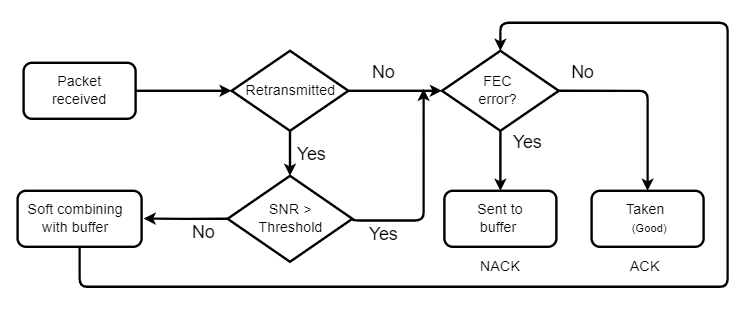
\includegraphics[width=0.8\textwidth]{sf.png}
    \caption{Decision-making process for soft combining at the receiver.}
    \label{fig:8}
\end{figure}

Figure \ref{fig:8} shows the decision-making process for soft combining. After receiving a packet, the receiver performs the following three steps:

% \begin{enumerate}
% \item[Step 1,] \textit{Packet Classification:} \\
% The receiver first determines whether the packet is an original transmission or a retransmission. This is critical for subsequent processing decisions.

% \item[Step 2,] \textit{SNR Estimation:} \\
% The EVM algorithm calculates the SNR of the received signal. Based on this estimation:

% \begin{itemize}
%     \item \textit{High SNR:} If the SNR exceeds a predetermined threshold, it indicates strong signal quality. Since the signal is probably error-free, the packet is routed straight to the error detection module without soft combining. Unnecessarily combining such high-quality signals with buffered data may reduce decoding accuracy.
    
%     \item \textit{Low SNR:} The signal quality is poor if the SNR drops below the threshold. In this case, the retransmitted packet is integrated with previously buffered data using soft combining, which increases decoding reliability by utilizing cumulative information from numerous receptions.
% \end{itemize}

% \item[Step 3,] \textit{Error Detection and Feedback :}
% \begin{itemize}
%     \item If the receiver correctly decodes the combined packet and finds it error-free, it accepts the packet.
    
%     \item If errors continue to occur, the receiver sends a NACK to request more retransmissions and keeps the packet buffered.
% \end{itemize}
% \end{enumerate}


\subsubsection{Packet Classification} 
\vspace{-0.03in}
The receiver first determines whether the packet is an original transmission or a retransmission. This is critical for subsequent processing decisions.

\vspace{-0.1in}

\subsubsection{SNR Estimation} 
\vspace{-0.03in}
The EVM algorithm calculates the SNR of the received signal. Based on this estimation:

\begin{itemize}
    \item \textit{High SNR:} If the SNR exceeds a predetermined threshold, it indicates strong signal quality. Since the signal is probably error-free, the packet is routed straight to the error detection module without soft combining. Unnecessarily combining such high-quality signals with buffered data may reduce decoding accuracy.
    \item \textit{Low SNR:} The signal quality is poor if the SNR drops below the threshold. In this case, the retransmitted packet is integrated with previously buffered data using soft combining, which increases decoding reliability by utilizing cumulative information from numerous receptions.
\end{itemize}

\vspace{-0.15in}

\subsubsection{Error Detection and Feedback}
\vspace{-0.03in}
\begin{itemize}
    \item If the receiver correctly decodes the combined packet and finds it error-free, it accepts it.
    
    \item If errors continue to occur, the receiver sends a NACK to request more retransmissions and keeps the packet buffered.
\end{itemize}


% \vspace{0.4cm}
%  \tcbox[colframe=black, colback=gray!20, sharp corners, boxrule=0.5pt, left=3pt, right=3pt, top=1pt, bottom=1pt]{\textbf{Step-1: Packet Classification}} The receiver first determines whether the packet is an original transmission or a retransmission. This is critical for subsequent processing decisions.

% \vspace{0.2cm}

% \tcbox[colframe=black, colback=gray!20, sharp corners, boxrule=0.5pt, left=3pt, right=3pt, top=1pt, bottom=1pt]{\textbf{Step-2 : SNR Estimation}} The EVM algorithm calculates the SNR of the received signal. Based on this estimation:

% \begin{itemize}
%     \item \textit{High SNR:} If the SNR exceeds a predetermined threshold, it indicates strong signal quality. Since the signal is probably error-free, the packet is routed straight to the error detection module without soft combining. Because of needless redundancy, combining such high-quality signals with buffered data may reduce decoding accuracy.
    
%     \item \textit{Low SNR:} The signal quality is poor if the SNR drops below the threshold. In this case, the retransmitted packet is integrated with previously buffered data using soft combining, which increases decoding reliability by utilizing cumulative information from numerous receptions.
% \end{itemize}

% \vspace{0.2cm}

% \noindent \tcbox[colframe=black, colback=gray!20, sharp corners, boxrule=0.5pt, left=3pt, right=3pt, top=1pt, bottom=1pt]{\textbf{Step-3 : Error Detection and Feedback}}   If the receiver correctly decodes the combined packet and finds it error-free, it accepts the packet. If errors continue to occur, the receiver sends a NACK to request more retransmissions and keeps the packet buffered.

% \vspace{0.2cm}

The selective application of soft combining balances computational efficiency and decoding performance. Dynamically adapting to channel conditions enhances throughput and minimizes overall retransmission overhead.

\section{Results and Analysis} \label{s4}

Simulations of D-HARQ were conducted within the Land Mobile and Satellite (LMS) channel using MATLAB (version R2023a) and Python (version 3.10), focusing on rural and suburban environments. LMS channel facilitates communication between land-based mobile stations and satellites, enabling wide geographic coverage for services such as GPS, satellite phones, and remote sensing in remote or rural areas. Under these conditions, the energy loss in the Line of Sight (LOS) wave is comparatively insignificant. LOS is an unobstructed path between transmitter and receiver, offering reliable communication with minimal signal attenuation, which is crucial for applications like microwave links and satellite communication.

\begin{table}[!htbp]
\caption{Number of information and redundancy bits for various schemes}
\label{tab:2}
\centering
\small
\renewcommand{\arraystretch}{1.5} 
\begin{tabularx}{\columnwidth}{|>{\raggedright\arraybackslash}X|>{\raggedright\arraybackslash}X|>{\raggedright\arraybackslash}X|} \hline
    \textbf{Scheme} & \textbf{Information bits} & \textbf{Redundancy bits} \\ \hline
    ARQ & 4567 & 32 (CRC) \\ \hline
    HARQ1 with BCH codes & 3447 & 1152 \\ \hline
    HARQ2 with BCH codes & 2295 & 2304 \\ \hline
\end{tabularx}
\end{table}

Table \ref{tab:2}  details the number of information bits and the associated redundancy bits, such as CRC for ARQ and error-correcting bits for HARQ1 and HARQ2. This information illustrates the error correction capabilities of each scheme in communication systems. Additionally, Table \ref{tab:1} illustrates the simulation environment. Consequently, signal propagation in this context follows a lognormal distribution, characterized by its probability density function (PDF) \cite{r27}, as detailed below:

\begin{equation}
f(x) = \frac{e^{-\left(\frac{(\ln x)^2}{2\sigma^2}\right)}}{x\sigma\sqrt{2\pi}}
\end{equation}

For x $>$ 0, Where x represents the random variable for signal strength and $\sigma$ denotes the distribution of additive white Gaussian noise (AWGN).


\begin{table}[!htbp]
\caption{Simulation environment and parameters}
\label{tab:1}
\centering
\small
\renewcommand{\arraystretch}{1.5}
\setlength\tabcolsep{4pt} 
\begin{tabularx}{\columnwidth}{|>{\raggedright\arraybackslash}X|>{\raggedright\arraybackslash}X|} \hline
    \textbf{Parameters} & \textbf{Values} \\ \hline
    Channel model & Land, Mobile, and Satellite \\ \hline
    Channel conditions & Rural and Suburban \\ \hline
    ARQ Scheme & ARQ, HARQ1, HARQ2  \\ \hline
    No. of symbols in each block/packet & 511 \\ \hline
    No. of bits per symbol &  9  \\ \hline
    Delay & 5 $\times$ No. of information symbols \\ \hline
    Noise & White Gaussian (AWGN) noise  \\ \hline
    Simulation output & MATLAB (version R2023a) and Python (version 3.10)   \\ \hline
    Simulated SNR range & 0-18 dB \\ \hline  
\end{tabularx}
\vspace{0.1in}
\end{table}


Figure \ref{fig:7} illustrates a graph of a D-HARQ model, highlighting the thresholds for transitioning between different modes, established through a trial-and-error methodology. The simulations use various sets of thresholds. Ultimately, the graph aligns almost perfectly with the ideal curve for $\alpha1$ = 10, $\alpha2$ = $\beta$ = W = 64, where the ideal curve's throughput at a given SNR is expressed as:

\begin{equation}
    \eta_{\text{ideal}} = \max(\eta_{\text{ARQ}}, \eta_{\text{HARQ1}}, \eta_{\text{HARQ2}})
\end{equation}

Figure \ref{fig:7} demonstrates the performance benefits of implementing an adaptive HARQ strategy within the SNR range of 3.47 dB to 9 dB, compared to a traditional GBN approach. Adopting the D-HARQ method in this specific SNR interval substantially increases throughput, achieving a gain of approximately  $2.16\times 10^{16}$ times. Moreover, Figure \ref{fig:7} highlights the enhanced throughput achieved by utilizing two different states of HARQ, each configured with BCH codes of varying code rates. A notable throughput enhancement of 31.67\% is observed when transitioning from HARQ state 2 to HARQ state 1 within the SNR range of 6.68 to 12.89 dB. 

The D-HARQ model recommends transitioning from HARQ back to ARQ at higher SNR values, a strategy convincingly supported by the simulation curve. This curve demonstrates the necessity for such a switch, highlighting a significant improvement of about 28.5\% in throughput above 12.89 dB.

\begin{figure}[H]
    \centering
    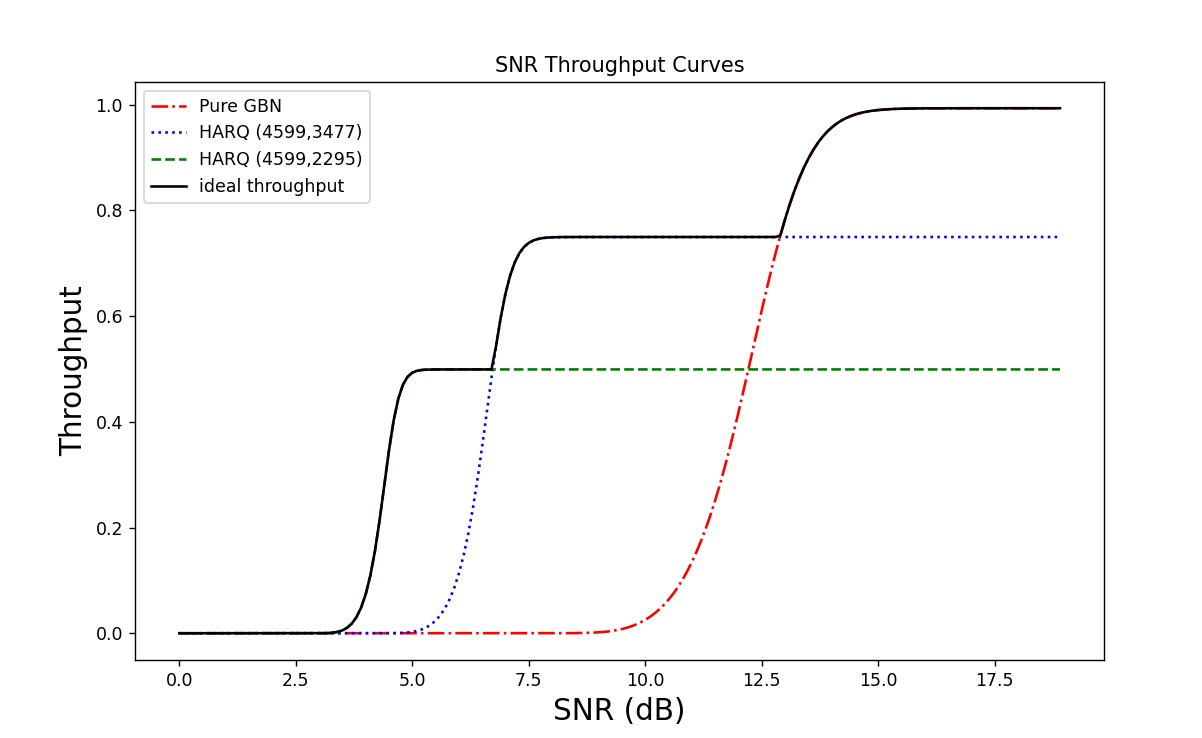
\includegraphics[width=\textwidth]{bch.jpg}
    \caption{Transitions between various HARQ and ARQ schemes}
    \label{fig:7}
\end{figure}

The main drawback observed from Fig \ref{fig:7} is negligible throughput nearing zero in the 0 to 3.47dB range. This D-HARQ model successfully avoids this by adapting HARQ with turbo codes in this range.

Figure \ref{fig:6} shows considerable throughput even at low SNR values, thus an improvement in throughput from 0 to 0.467 bpcu (bits per channel use) by adapting turbo codes. In Figure \ref{fig:6}, one might question the feasibility of utilizing turbo codes across all SNR ranges. Implementing Turbo Codes, while offering superior error correction capabilities, particularly in environments with a high SNR, presents a more complex challenge than BCH codes due to several key factors. The design of Turbo Codes especially includes a complex iterative decoding process that relies on information being passed back and forth between two or more constituent decoders. This interaction necessitates a complicated algorithm to properly converge on the correct decoding, greatly complicating implementation compared to the simple algebraic decoding methods employed for BCH codes.

As explained in Section \ref{s2}, Soft combining is beneficial as combining the retransmitted packet with the error packets in the buffer improves its decoding capability, thus reducing the need for retransmissions. However, at a very high SNR, soft combining does not contribute much towards the throughput improvement. Since these schemes are unnecessary in such scenarios, they are not employed, optimizing the complexity and minimizing the usage of resources.

\begin{figure}[H]     
    \centering     
    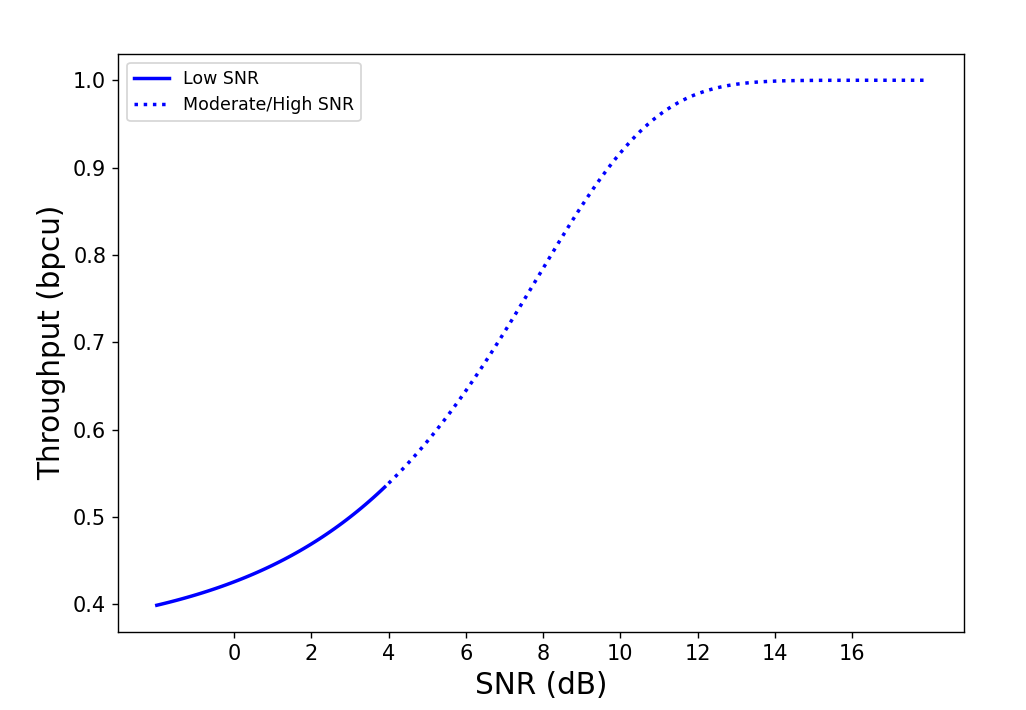
\includegraphics[width= 0.9 \textwidth, height=8cm]{turbo_code.png}     
    \caption{Estimated Throughput vs SNR for HARQ with Turbo codes (code rate = 1/3)}     
    \label{fig:6} 
\end{figure}


Figure \ref{fig:9} compares throughput with and without soft combining at all SNR values ranging from 0 to 50 dB. Thus, the threshold to selectively soft combine is 17.46 dB. Therefore, an SNR above this threshold indicates that the channel quality is good enough to omit soft combining.

Although D-HARQ introduces added complexity through dynamic switching, turbo code integration, and selective soft combining, these features are essential for significantly improving performance, particularly in low SNR conditions (0–3.47 dB). The system’s ability to adapt to changing channel conditions and minimize retransmissions boosts throughput and resource efficiency.  For instance, turbo codes improve throughput from 0 to 0.467 bpcu, as shown in Figure \ref{fig:6}, and adaptive HARQ outperforms traditional GBN in the 3.47 dB to 9 dB SNR range, as seen in Figure \ref{fig:7}. Furthermore, selective soft combining is only applied when SNR is below 17.46 dB, ensuring optimal use of resources.

\begin{figure}[H]
    \centering
    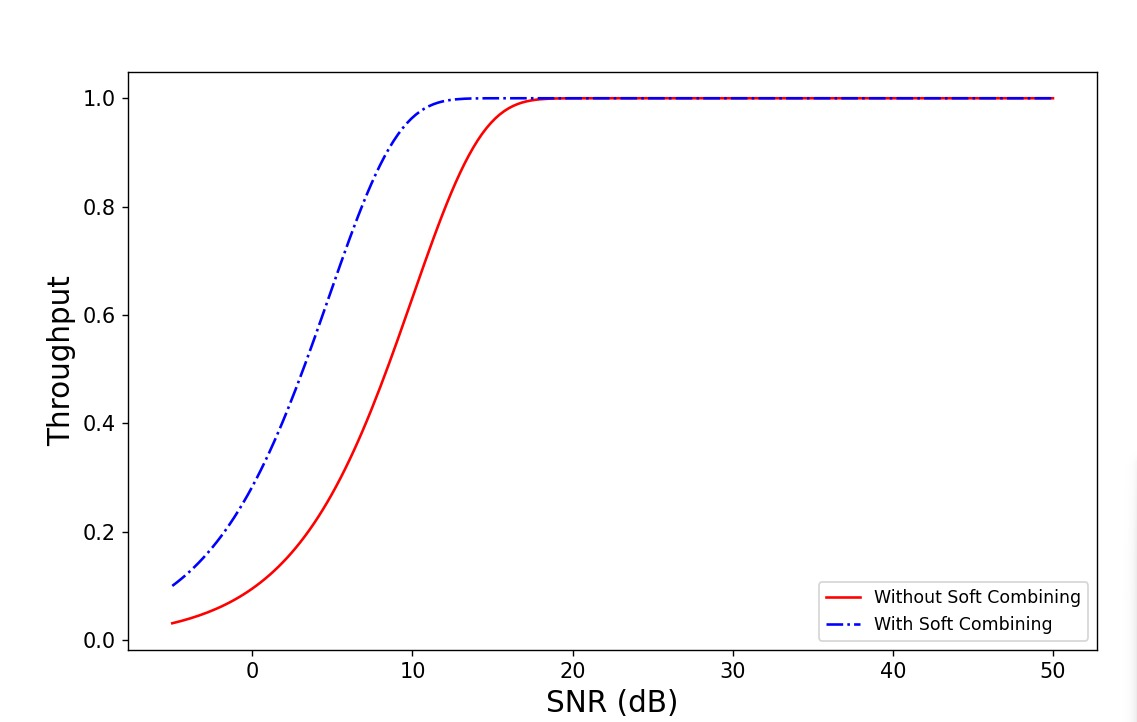
\includegraphics[width=0.9 \textwidth, height = 8cm]{soft_combining.jpg}
    \caption{Performance comparison with and without Soft combing}
    \label{fig:9}
\end{figure}


\section{Conclusion and Future Works} \label{s5}

This paper introduced D-HARQ, an SNR-responsive scheme that switches between ARQ and HARQ using BCH and turbo coding. Additionally, the selective soft combining method integrates with it to improve performance. The strategic utilization of turbo codes under very low SNR conditions and BCH codes in other scenarios strike an optimal balance between cost-effectiveness and reliability. Soft combining is purposely avoided during favorable channel conditions, reducing the related complexity overhead. Moreover, enhancing performance and throughput. Simulation results that employ turbo coding and selective soft combining confirm the usefulness of this paper's idea. These findings show a significant gain in throughput while lowering complexity at all levels of data transmission. Future work could include simulations using machine learning approaches to determine proper thresholds. Future research can focus on finding ways to deliver high throughput while maintaining low latency. 

\newpage

\section*{\textbf{Statements \& Declarations}}

\subsection*{Competing Interests}
I have no conflicts of interest to disclose. No financial conflicts with any author
or agencies.

\subsection*{Funding}
The authors declare that no funds, grants, or other support were received during the preparation of this manuscript.

\subsection*{Author Contributions}
Material preparation and analysis were performed by us only.

\subsection*{Data availability statements (DAS)}
As our own

\subsection*{Research Involving Human and /or Animals}
As our own

\subsection*{Informed Consent}
Not applicable


\bibliography{reference}

\end{document}
